% https://tex.stackexchange.com/a/758838

\documentclass[tikz,border=5pt]{standalone}
\usetikzlibrary{decorations.markings}
\begin{document}

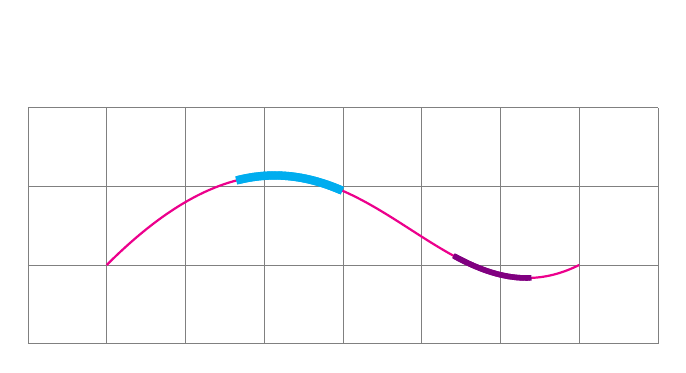
\begin{tikzpicture}
    \draw[help lines] (-1,-1) grid (7,2);
    \draw[
        thick,magenta,
        postaction=decorate,
        decoration={
            markings,
            mark=between positions 0.3 and 0.5 step 0.5pt
                with {\draw[line width=1pt,cyan] (0, -1.5pt) --(0, 1.5pt);},
            mark=between positions 0.75 and 0.9 step 0.5pt
                with {\draw[line width=1pt,violet] (0, -1pt) --(0, 1pt);},
            },
    ] 
    (0,0) .. controls (3,3) and (4,-1) .. (6,0);
\end{tikzpicture}

\end{document}
